\documentclass[12pt, a4paper, oneside]{ctexart}
\usepackage{amsmath, amsthm, amssymb, bm, color, framed, graphicx, hyperref, mathrsfs, mathtools, enumerate, tikz}
\usepackage{float}
\usepackage{subcaption} 



\usetikzlibrary{patterns}

\title{\textbf{Homework 8}}
\author{萃英学院\qquad 2022级\qquad 王一鑫}
\date{\today}
\linespread{1.5}
\newcounter{problemname}
\newenvironment{problem}{\begin{framed}\stepcounter{problemname}\par\noindent\textsc{Problem \arabic{problemname}. }}{\end{framed}\par}
\newenvironment{solution}{%
	\par\noindent\textsc{Solution. }\ignorespaces
}{%
	\hfill$\qed$\par
}
\newenvironment{note}{\par\noindent\textsc{Note of Problem \arabic{problemname}. }}{\\\par}

\begin{document}
	
	\maketitle
	
	\begin{problem}
		(Exercise 4.24)
		
		Show that the dual of the cube graph is the octahedron graph, 
		and that the dual of the dodecahedron graph is the icosahedron graph. 
		What is the dual of the tetrahedron graph?

    
	\end{problem}
    
	\begin{solution}
        
	    The cube has $8$ vertices, $12$ edges, and $6$ faces. 
		The octahedron has $6$ vertices, $12$ edges, and $8$ faces.

		The icosahedron has $12$ vertices, $30$ edges, and $20$ faces.
		The dodecahedron has $20$ vertices, $30$ edges, and $12$ faces.

		Apply lemma 4.12 we know that the dual of the cube graph is the octahedron graph, 
		and that the dual of the dodecahedron graph is the icosahedron graph. 

		The dual of the tetrahedron graph is itself the tetrahedron graph.

		
	\end{solution}
		

		
	
	\begin{problem}
		(Exercise 4.28)

        \begin{enumerate}
			\item[(i)] Give an example to show that, if $G$ is a disconnected plane graph, then $G^{**}$ is not isomorphic to $G$.
			\item[(ii)] Prove the result of part (i) in general.
		\end{enumerate}
		


	\end{problem}
	
	\begin{solution}
		
		\begin{enumerate}[(i)]
			\item Consider the graph \( G \) consisting of two disconnected components, where one component is a triangle (denoted by \( K_3 \)) and the other is a single vertex. Specifically, let \( G \) be the disjoint union of \( K_3 \) and a single vertex, denoted by \( v \). This graph is clearly disconnected.

			Then $G$, $G^{*}$ and $G^{**}$ is shown in Fig \ref{fig:ex1}. We can easily check that $G^{**}$ is not isomorphic to $G$.

			\begin{figure}[H]
				\small
				\centering
				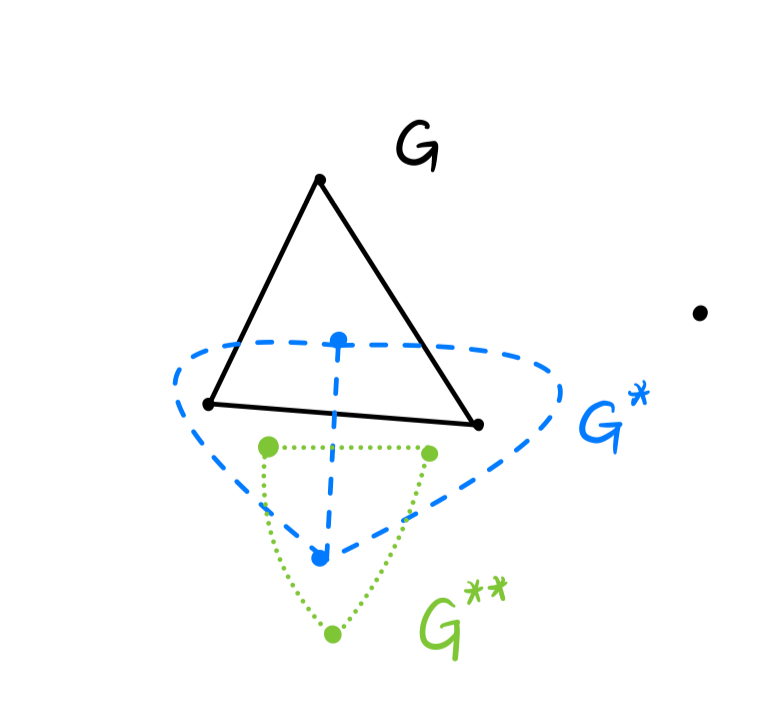
\includegraphics[width=0.5\columnwidth]{figure/fig1.jpg}
				\caption{Example}
				\label{fig:ex1}
			\end{figure}
			\item Similar with the proof of Theorem 4.13. However, Euler formula doesn't
			hold in disconnected graph, thus we can't assure that a face of $G^{*}$ contain only
			one vertex of $G$, so $G^{**}$ is not isomorphic to $G$.
		\end{enumerate}

	\end{solution}
	
	\begin{problem}
        (Exercise 4.30)

		Prove that, if $G$ is a 3-connected plane graph, then its geometric dual 
		is a simple graph.

       
	\end{problem}
	
	\begin{solution}
       
        If $G$ is 3-connected, then $G$ has no vertices of degree 1 or 2, and hence $G^*$ has no loops or multiple edges, and is therefore a simple graph.

        
	\end{solution}
	
	
	
	\begin{problem}
        (Exercise 4.31) 
        
		Let $G$ be a connected plane graph. Using Theorem 2.1 and Corollary 2.10, 
		prove that $G$ is bipartite if and only if its dual $G^*$ is Eulerian.
		(This result will be needed in Chapters 5 and 7.)

		
	\end{problem}
	
	\begin{solution}
        
        If $G$ is bipartite, then each cycle of $G$ has even length, 
		and thus each cutset of $G^*$ has an even number of edges; 
		in particular, each vertex of $G^*$ has even degree, 
		and thus $G^*$ is Eulerian. The reverse implication is obtained 
		by reversing the argument.

		
	\end{solution}


	\begin{problem}
		(Exercise 4.32)

		\begin{enumerate}
			\item[(i)] Give an example to show that, if $G$ is a connected plane graph, then any spanning tree in $G$ corresponds to the complement of a spanning tree in $G^*$.
			\item[(ii)] Prove the result of part (i) in general.
		\end{enumerate}
		(This result will also be needed in Chapter 7.)		
        
        
    \end{problem}

	\begin{solution}
       
		\begin{enumerate}[(i)]
			\item Consider a triangle graph $G$ with three vertices and three edges 
			forming a cycle. The dual graph $G^*$ has two vertices 
			(one for each face, inside and outside the triangle) connected by three 
			edges, each corresponding to an edge of $G$. Let $T$ be a spanning tree 
			in $G$ consisting of any two edges, say $e_1$ and $e_2$. 
			The complement of $T$ in $G$ is the edge $e_3$. In $G^*$, 
			a spanning tree $T^*$ must connect the two vertices, 
			which requires one edge. If we take $T^*$ to be the edge corresponding 
			to $e_3$ in $G$, then the complement of $T$ in $G^*$ consists of the edges 
			corresponding to $e_1$ and $e_2$. Thus, the edges of $T$ in $G$ correspond 
			to the complement of $T^*$ in $G^*$, illustrating the result. It is shown in Fig \ref{fig:ex2}.
			\begin{figure}[H]
				\small
				\centering
				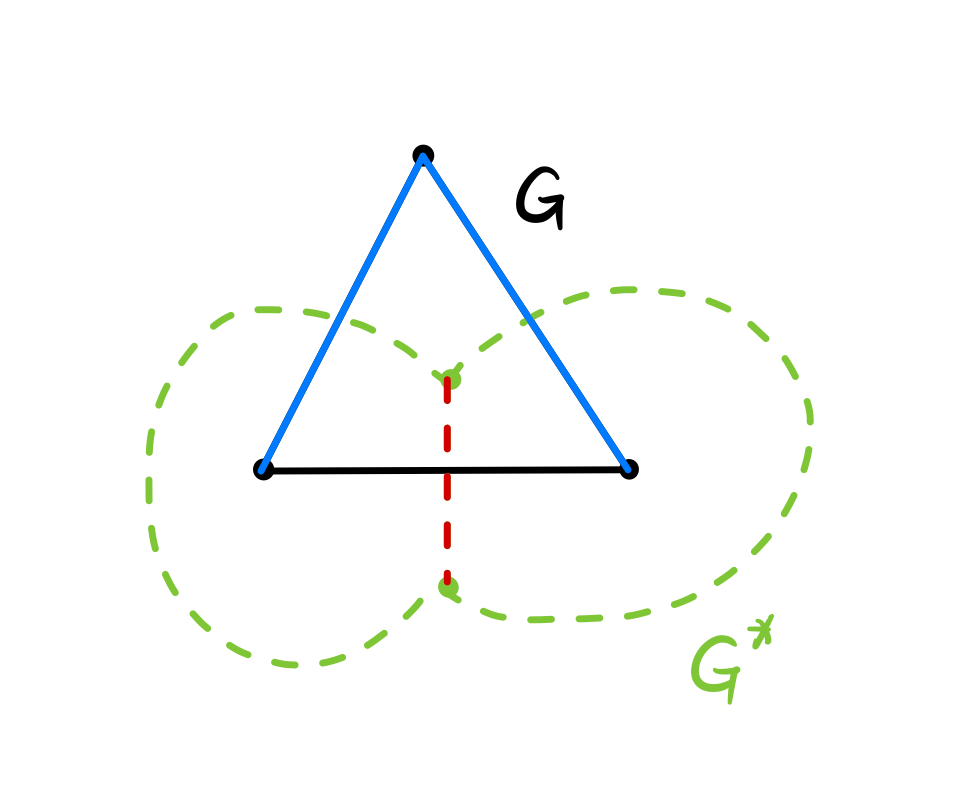
\includegraphics[width=0.5\columnwidth]{figure/fig2.jpg}
				\caption{Example}
				\label{fig:ex2}
			\end{figure}

			\item 
				First for a connected planar graph $G$ with $|V|$ vertices, $|E|$ edges, 
				and $|F|$ faces, Euler's formula gives $|V| - |E| + |F| = 2$. 
				The dual graph $G^*$ has $|F|$ vertices. A spanning tree in $G$ has $|V| - 1$ 
				edges, so the complement has $|E| - (|V| - 1) = |E| - |V| + 1$ edges. 
				A spanning tree in $G^*$ requires $|F| - 1 = (|E| - |V| + 2) - 1 = |E| - |V| + 1$ 
				edges, matching the complement edge count.
			
				Now suppose the complement of a spanning tree $T$ in $G$ is disconnected in $G^*$. 
				This implies a partition of $G^*$'s vertices (faces of $G$) with no connecting edges in the complement, meaning all such edges are in $T$. This contradicts $T$ being a tree, as it would imply a disconnecting set in $T$.
			
				A cycle in $G^*$ corresponds to a minimal cut in $G$. If the complement of $T$ had a cycle, the corresponding cut in $G$ would be entirely in the complement, contradicting $T$'s connectedness.
			
		\end{enumerate}


    \end{solution}
		
    
	\begin{problem}
		(Exercise 4.34)

		Using the representation in Exercise 4.33, show that the Petersen graph has genus 1.

    \end{problem}

	\begin{solution}
       Shown in Fig \ref{fig:petersen}.
	   \begin{figure}[H]
		\small
		\centering
		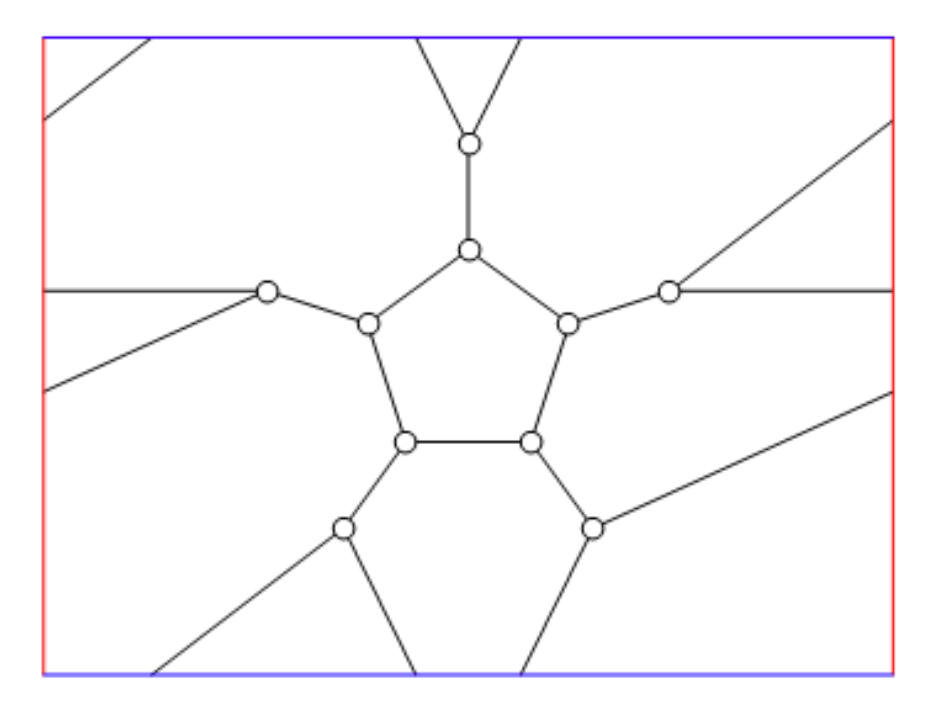
\includegraphics[width=0.45\columnwidth]{figure/fig3.png}
		\caption{Representation}
		\label{fig:petersen}
	\end{figure}
		
	\end{solution}


	\begin{problem}
		(Exercise 4.36)
        
		\begin{enumerate}
			\item[(i)] Use Theorem 4.21 to prove that there is no value of $n$ for which $g(K_n) = 7$.
			\item[(ii)] What is the next integer that is not the genus of any complete graph?
		\end{enumerate}		
        

	\end{problem}

	\begin{solution}
        
		\begin{enumerate}[(i)]
			\item When $k = 12$, by the formula in Theorem 4.21
			\[g(K_n) = \lceil \dfrac{1}{12}(n-3)(n-4)\rceil\]
			there is no value of $n$ for which $g(K_n) = 7$.

			\item When $k = 14$, $g(K_n) = 10$. So the next integer that is not the genus of any complete graph is $9$.
		\end{enumerate}
    
	\end{solution}
     

    \begin{problem}
        (Exercise 4.37)

		\begin{enumerate}
			\item[(i)] Give an example of a plane graph that is regular of degree 4 and in which each face is a triangle.
			\item[(ii)] Show that there is no graph of genus $g \geq 1$ with these properties.
		\end{enumerate}		

       
    \end{problem}
	
    \begin{solution}
       
		\begin{enumerate}
			\item[(i)] The octahedron graph.
			\item[(ii)] For such a graph, $4n = 2m = 3f$. It follows from Theorem 4.19 that
			\[
			\frac{1}{2}m - m + \frac{2}{3}m = 2 - 2g,
			\]
			and so $m = 12(1 - g)$, which is not positive. This contradiction shows that no such graph can exist.
		\end{enumerate}
		
        
    \end{solution}

    \begin{problem}
        (Exercise 4.38)

        \begin{enumerate}
			\item[(i)] Obtain a lower bound, analogous to that of Corollary 4.20, for a graph containing no triangles.
			\item[(ii)] Deduce that $g(K_{r,s}) \geq \left\lceil \frac{1}{4}(r-2)(s-2) \right\rceil$.
			(Ringel has shown that this is an equality).
		\end{enumerate}
		

    \end{problem}

    \begin{solution}
        
		\begin{enumerate}[(i)]
			\item Since each face is bounded by at least three edges, 
			we have $4f \leq 2m$ (as in the proof of Corollary 4.8(ii)). 
			The result follows on substituting this inequality into Theorem 4.19, 
			and using the fact that the genus of a graph is an integer, we have
			\[g(G)\geq \lceil\dfrac{1}{4}(m-2n)+1\rceil\]
			
			\item For $K_{r,s}$, there are $r+s$ vertices and $rs$ edges. Let $m = rs$ and 
			$n = r+s$ in (i) we have 
			\[g(G)\geq \lceil\dfrac{1}{4}(m-2n)+1\rceil = \lceil\dfrac{1}{4}(rs-2(r+s))+1\rceil = \lceil \frac{1}{4}(r-2)(s-2) \rceil\]

		\end{enumerate}
        
    \end{solution}
\end{document}


